\section{Initial and Revised Interface Design}

\subsection{Home}
\subsubsection{Initial}

\includegraphics[width=6in]{../other/initial-interface-design/home.png}
\subsubsection{Revised}
There will a paragraph introducing the lab and the participant scheduling system. Furthermore, it will explain who should be clicking what to get started. On every page, the menu button associated with the current page will be distinguished in some way.

\subsection{Sign Up}
\subsubsection{Initial}
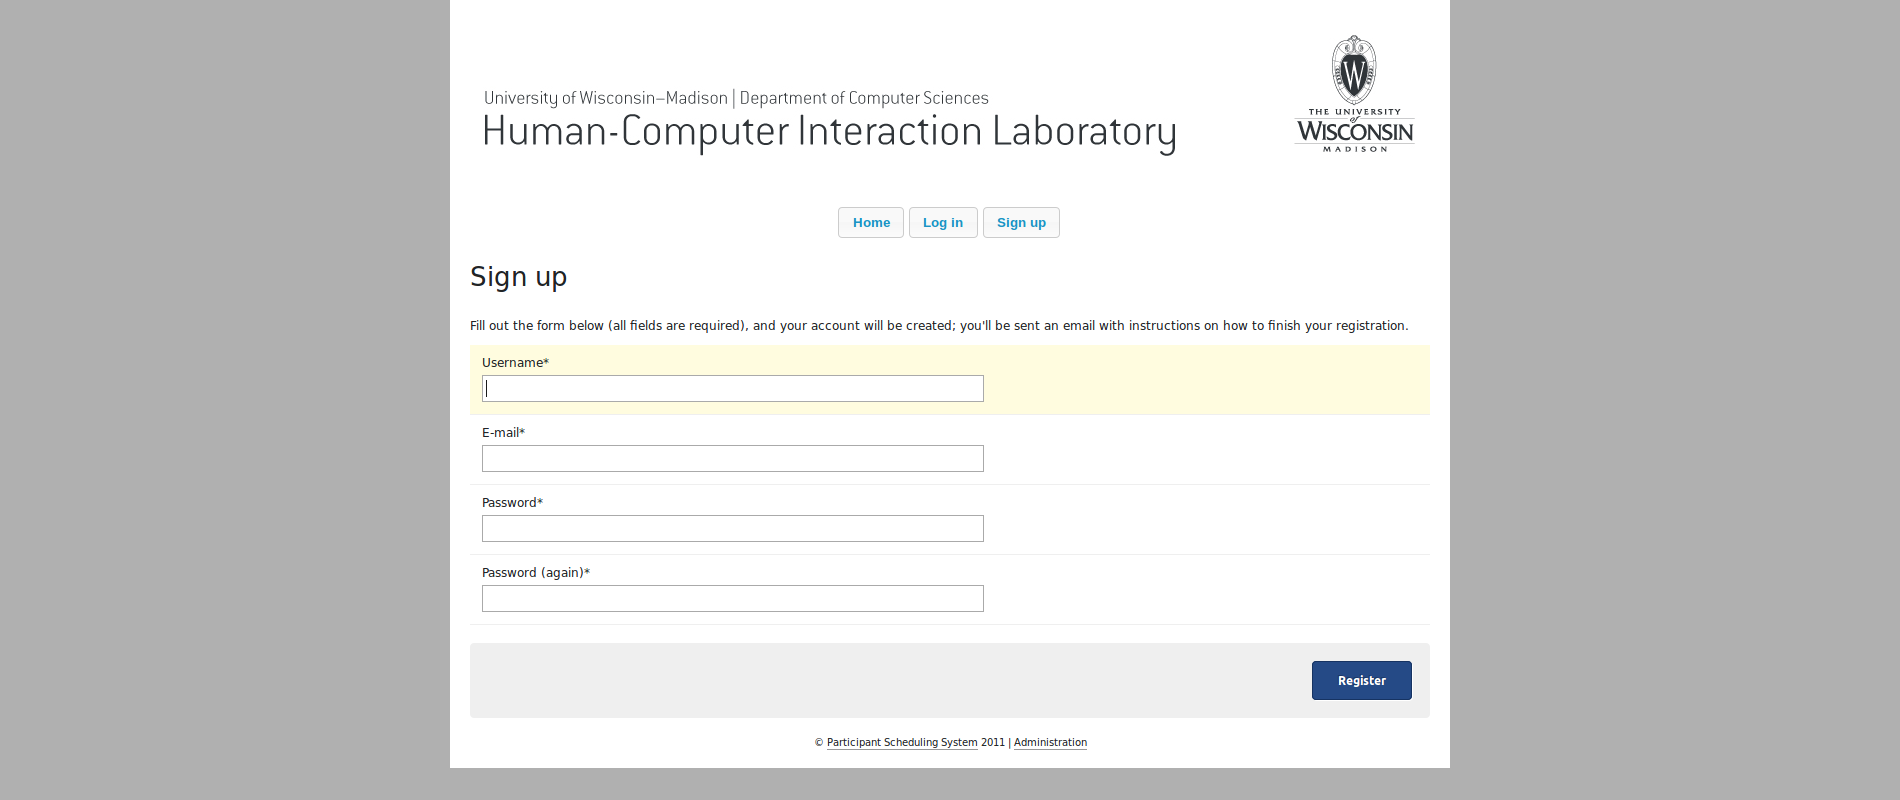
\includegraphics[width=6in]{../other/initial-interface-design/sign-up.png}
\subsubsection{Revised}
No changes

\subsection{Log In}
\subsubsection{Initial}
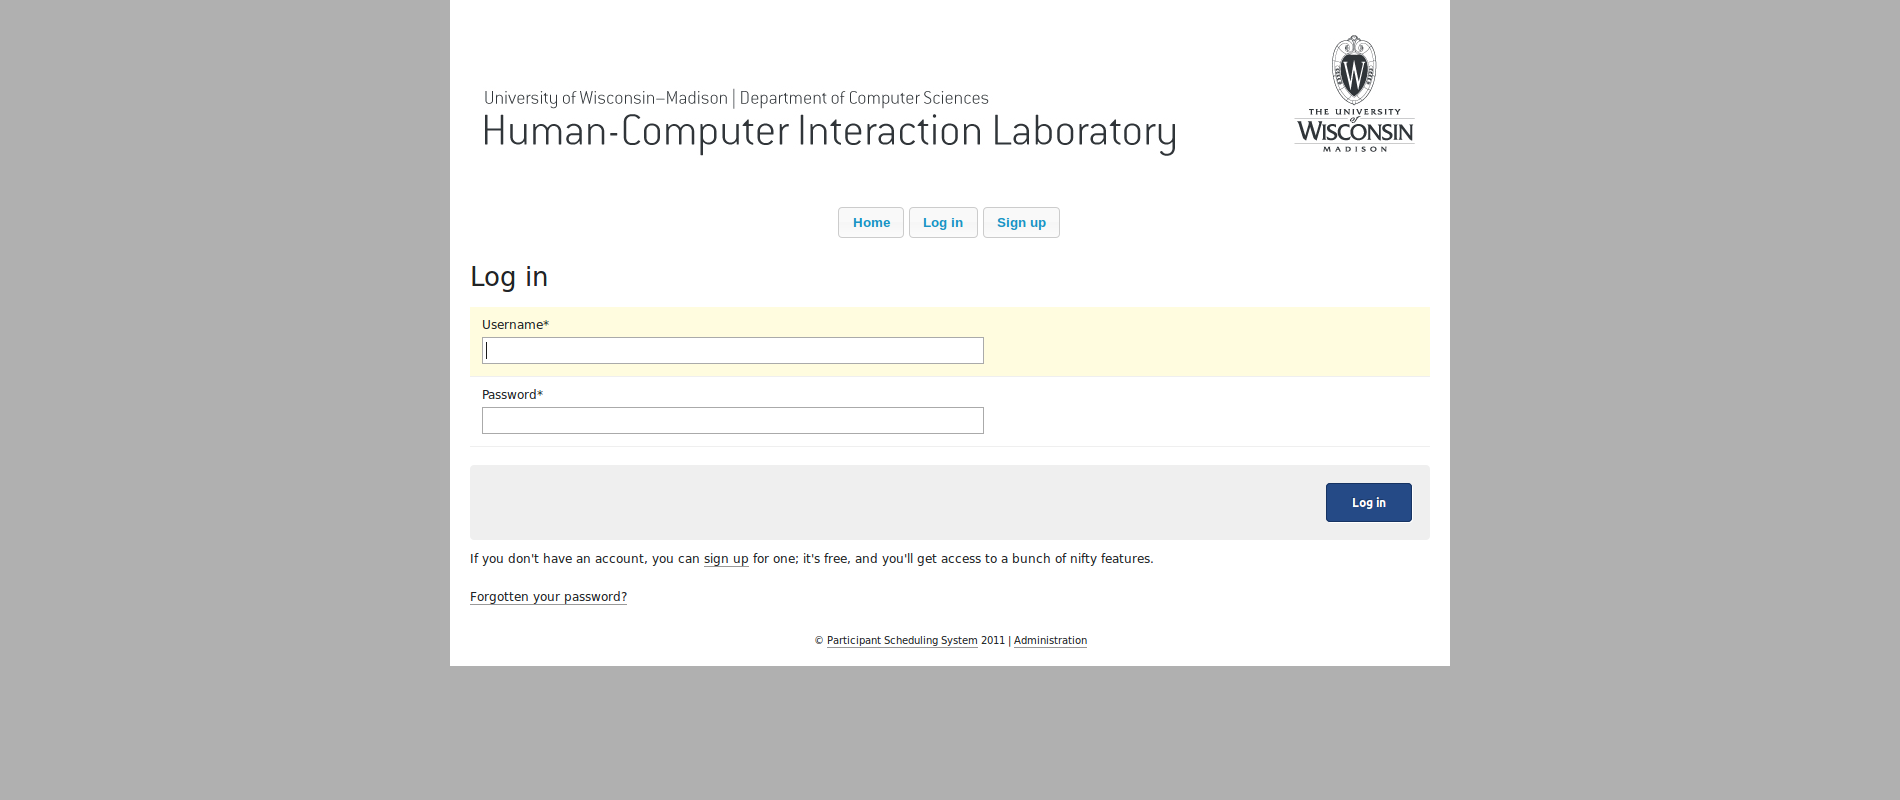
\includegraphics[width=6in]{../other/initial-interface-design/log-in.png}
\subsubsection{Revised}
No changes

\subsection{Password Reset}
\subsubsection{Initial}
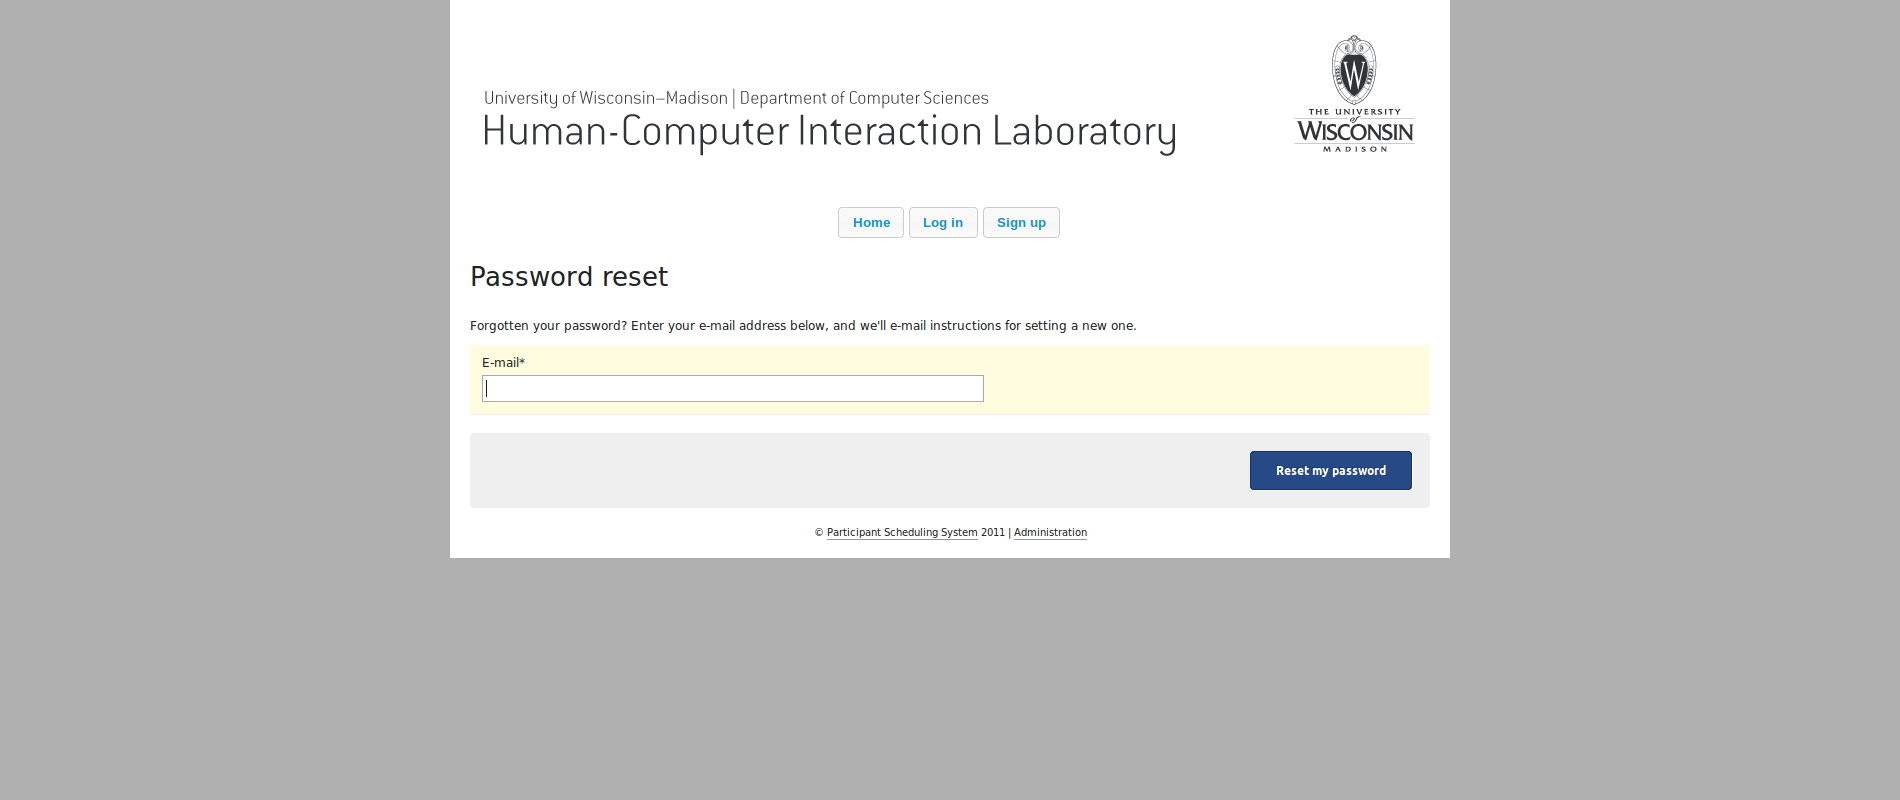
\includegraphics[width=6in]{../other/initial-interface-design/password-reset.png}
\subsubsection{Revised}
No changes

\subsection{Home, Logged In}
\subsubsection{Initial}

\includegraphics[width=6in]{../other/initial-interface-design/home-2.png}
\subsubsection{Revised}
Upon logging in, instead of being taken back to the home page, the user will be taken to the experiments page. If the user manually returns to the home page while logged in, the revisions of the default home page will be reflected there as well; see {\bf Home, Logged In}. On every page, the logged in user's username or name will be displayed somewhere.

\subsection{Password Change}
\subsubsection{Initial}
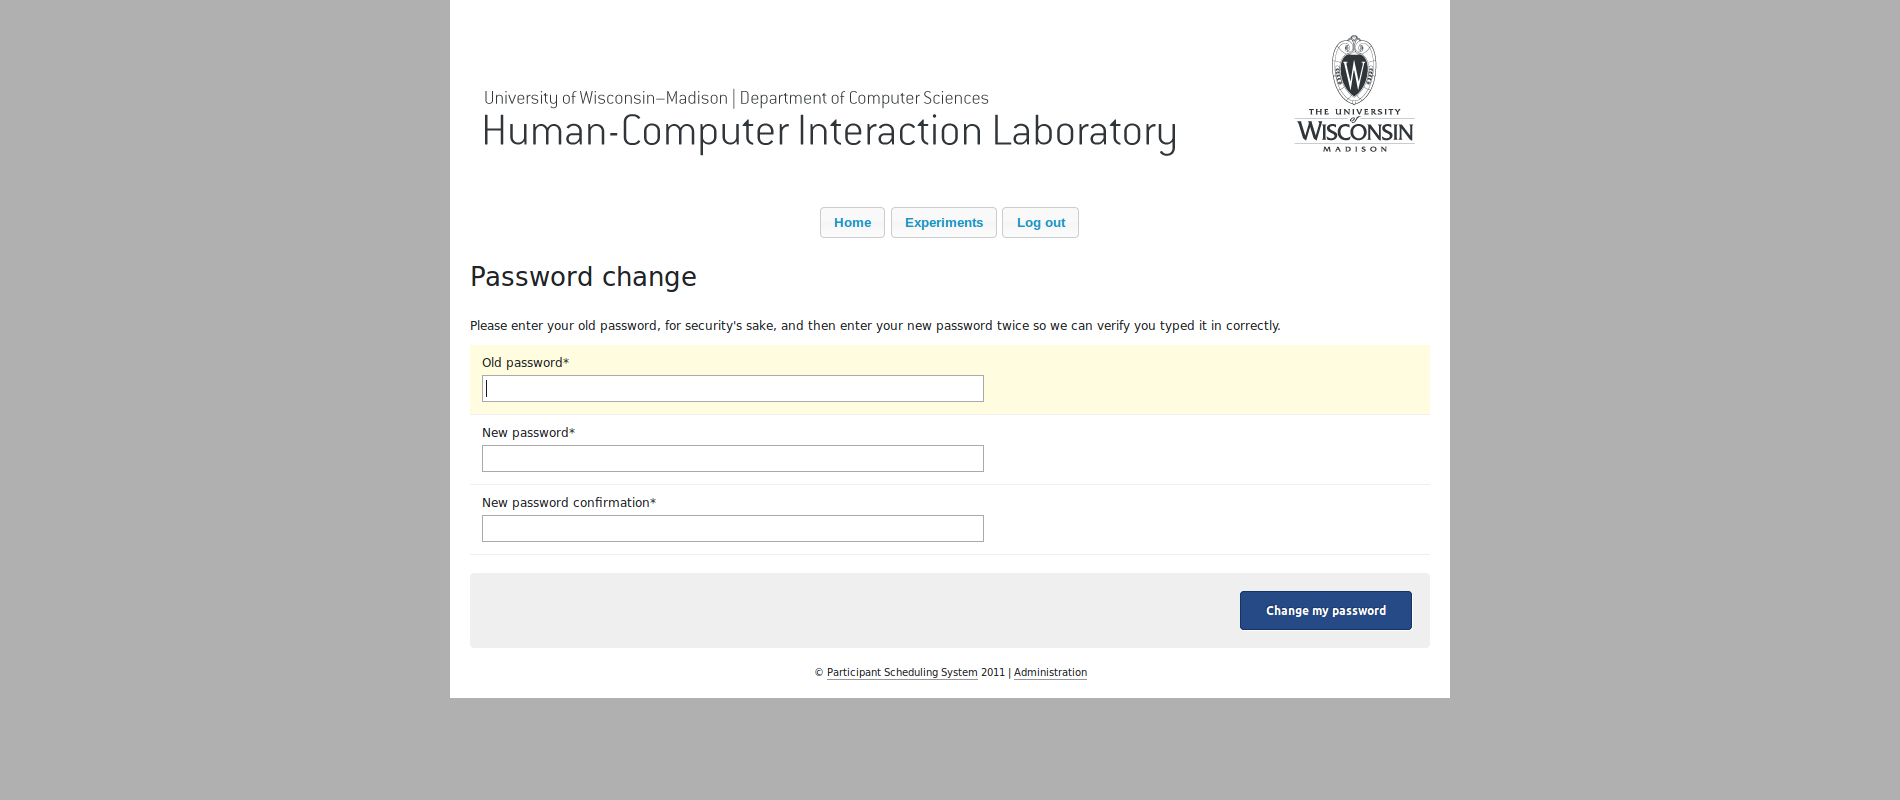
\includegraphics[width=6in]{../other/initial-interface-design/password-change.png}
\subsubsection{Revised}
It will be linked to from some other page, maybe the home page while logged in. No user was able to access it without explicitly visiting the URL, which they were not given.

\subsection{Experiments}
\subsubsection{Initial}
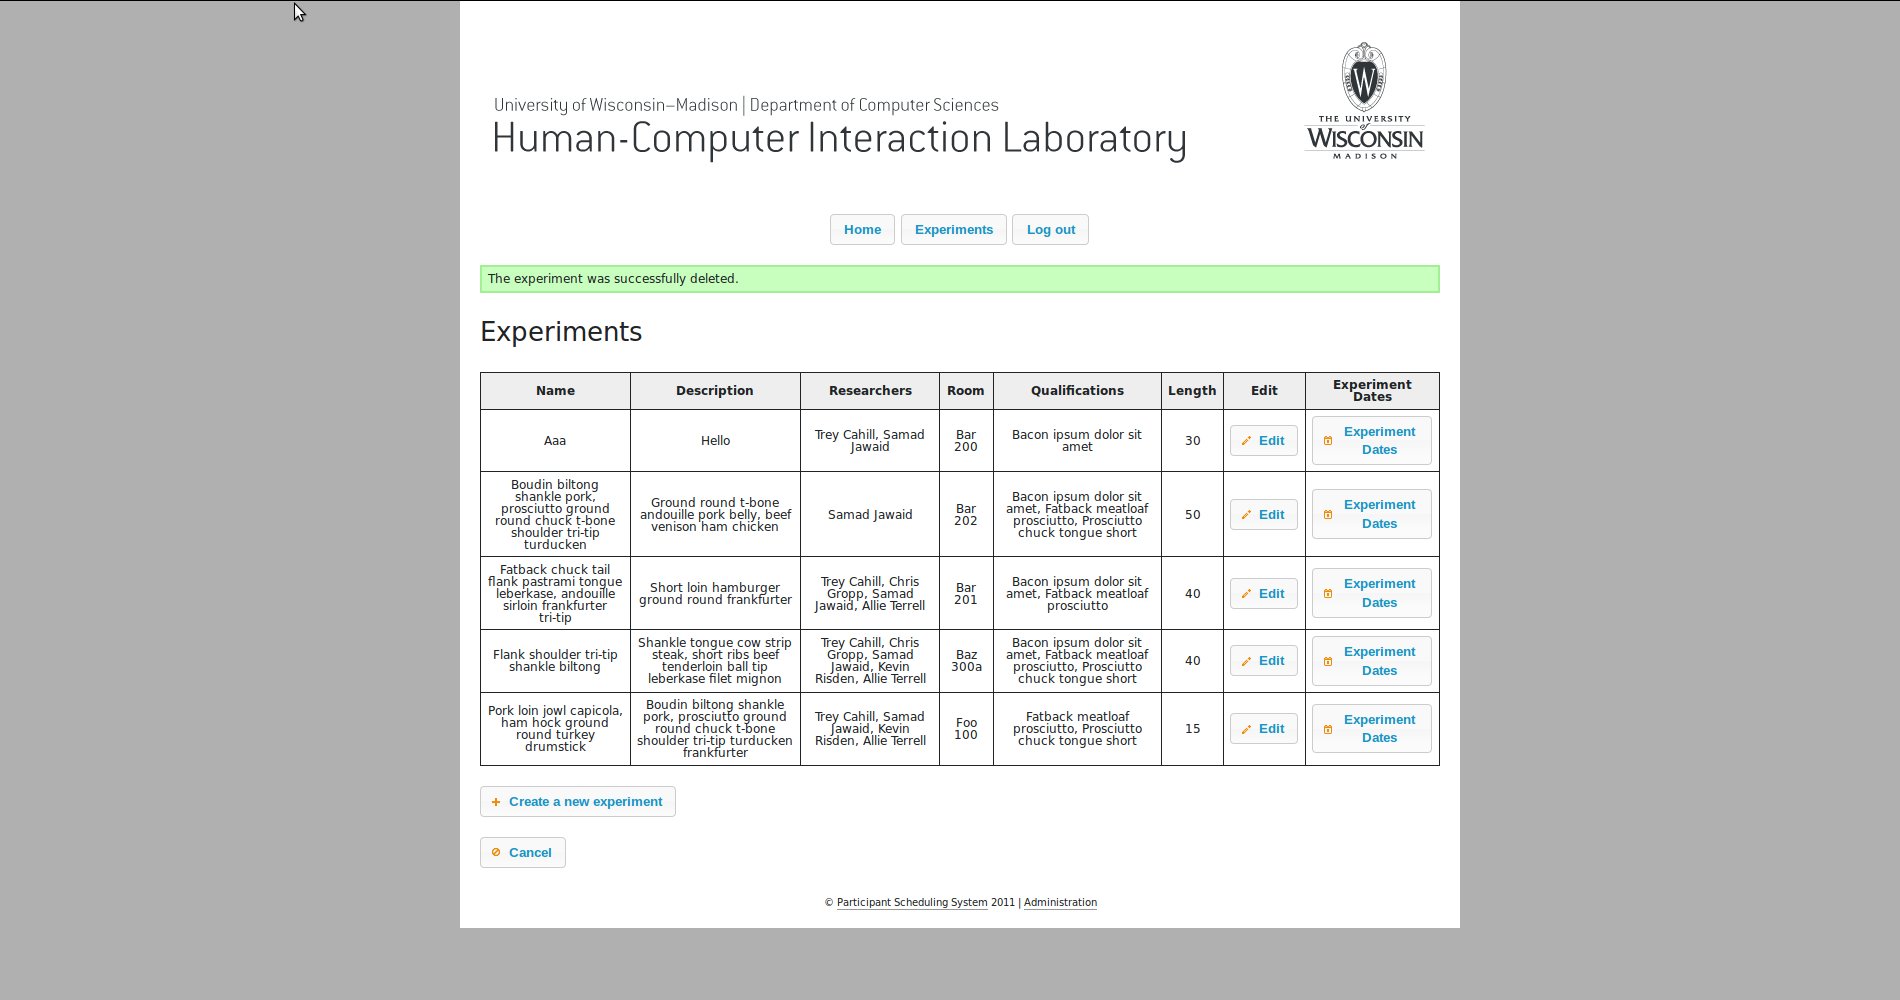
\includegraphics[width=6in]{../other/initial-interface-design/experiments.png}
\subsubsection{Revised}
The unit of length (minutes) will be specified. The table will be filterable and sortable. Experiments will be able to be mass-deleted from the table. The create button will be duplicated above the table as well. The cancel button will be changed to a back button with an appropriate icon.

\subsection{Create Experiment}
\subsubsection{Initial}
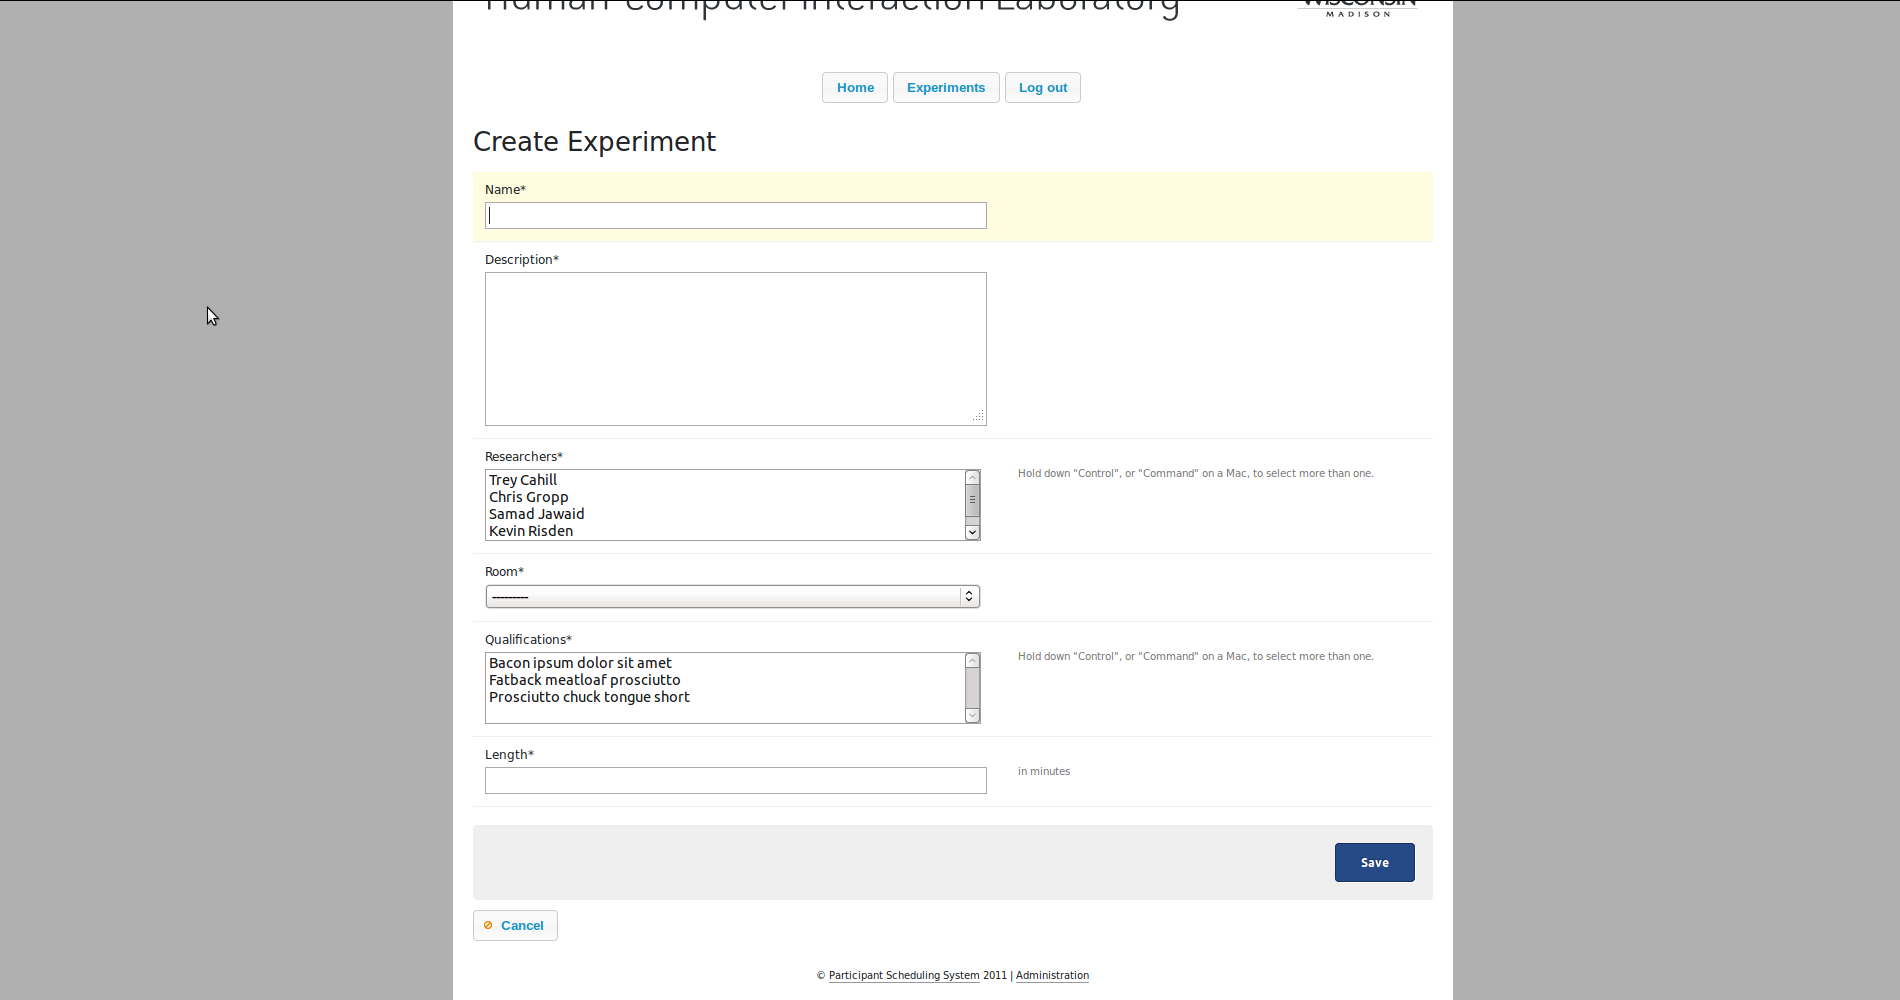
\includegraphics[width=6in]{../other/initial-interface-design/create-experiment.png}
\subsubsection{Revised}
The qualifications, room, and researchers inputs will be jQueryUI autocomplete fields with the ability to create new values. It will be clear that the cancel button discards all unsaved changes.

\subsection{Edit Experiment}
\subsubsection{Initial}
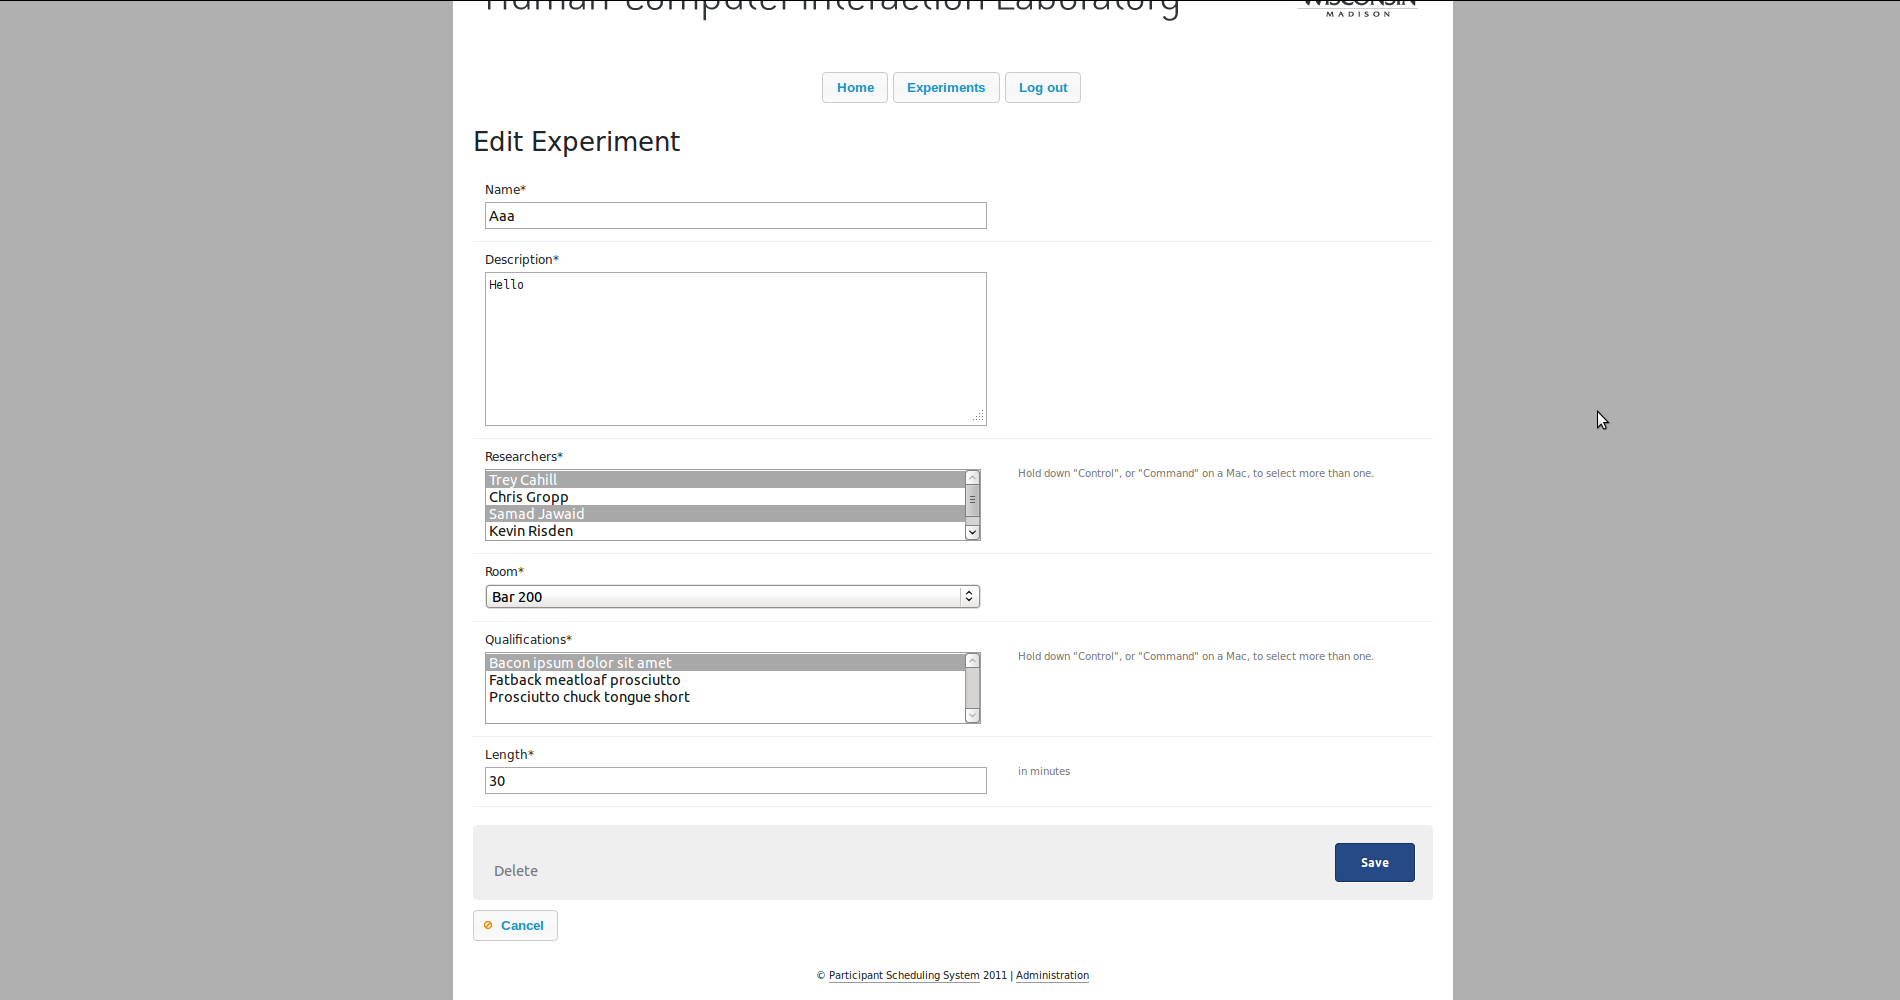
\includegraphics[width=6in]{../other/initial-interface-design/edit-experiment.png}
\subsubsection{Revised}
The delete button will not be so subtle. Also, see {\bf Create Experiment}.

\subsection{Delete Experiment}
\subsubsection{Initial}
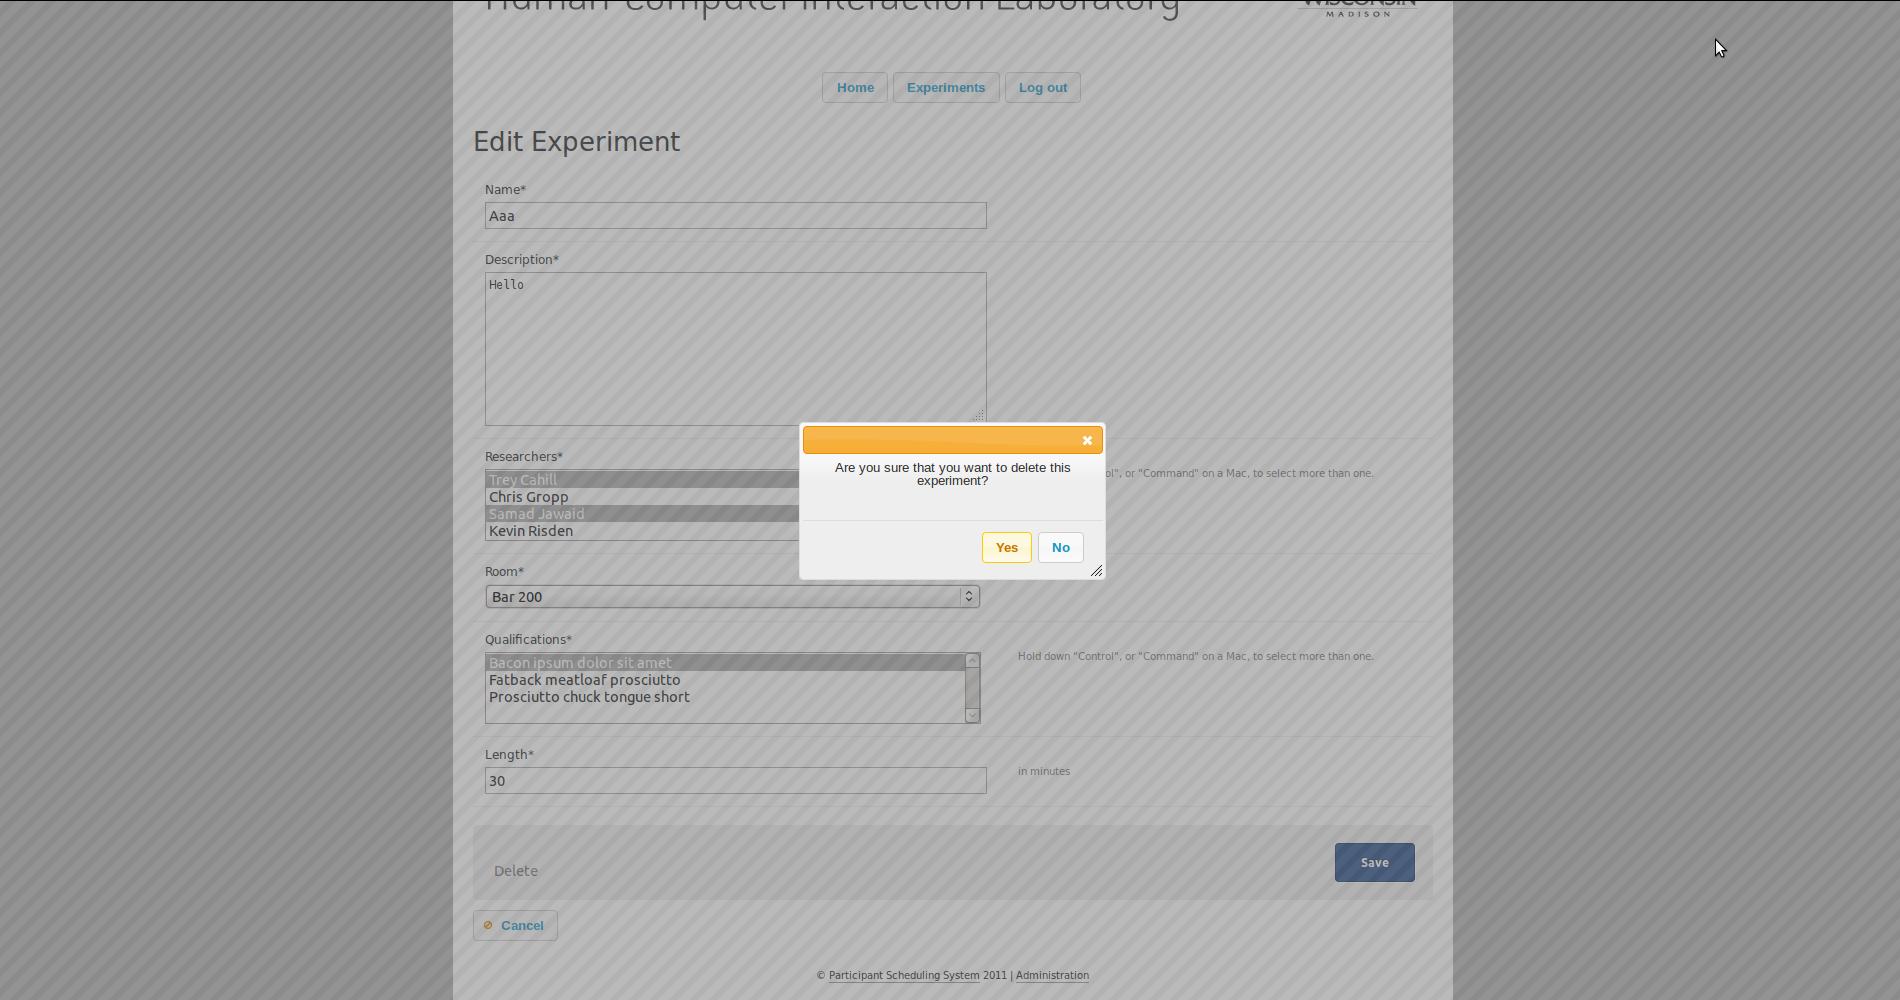
\includegraphics[width=6in]{../other/initial-interface-design/delete-experiment.png}
\subsubsection{Revised}
The jQueryUI CSS theme will match the existing CSS, so the dialog box will not appear so out of place.

\subsection{Experiment Dates}
\subsubsection{Initial}
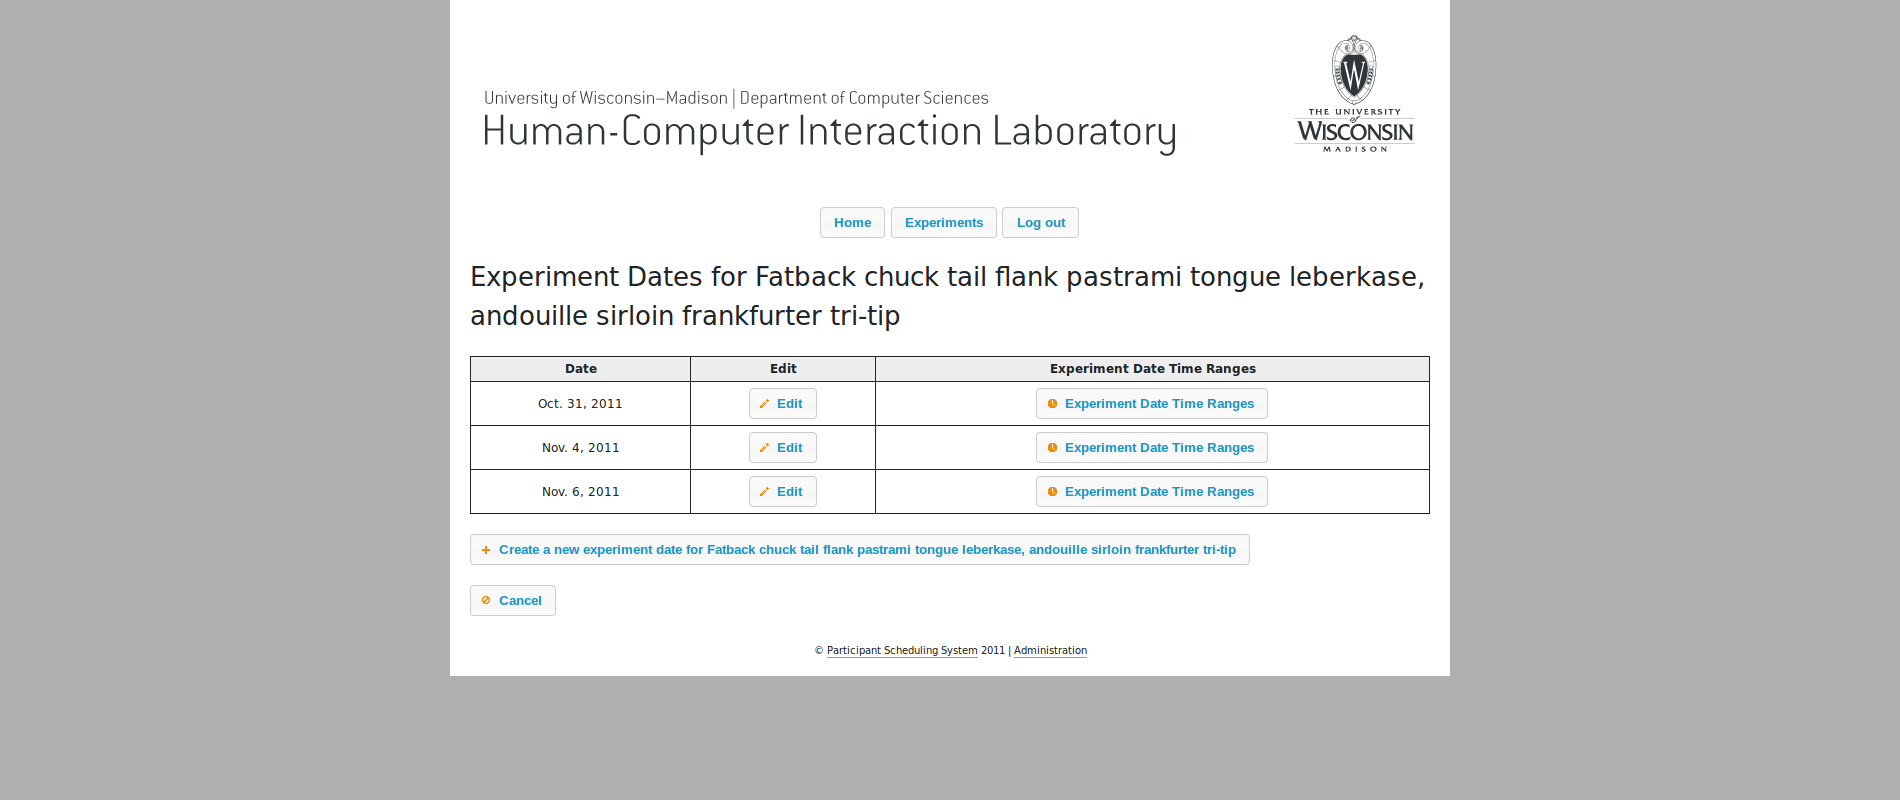
\includegraphics[width=6in]{../other/initial-interface-design/experiment-dates.png}
\subsubsection{Revised}
The table will be filterable and sortable. Experiment dates will be able to be mass-deleted from the table. The create button will be duplicated above the table as well. The cancel button will be changed to a back button with an appropriate icon.

\subsection{Create Experiment Date}
\subsubsection{Initial}
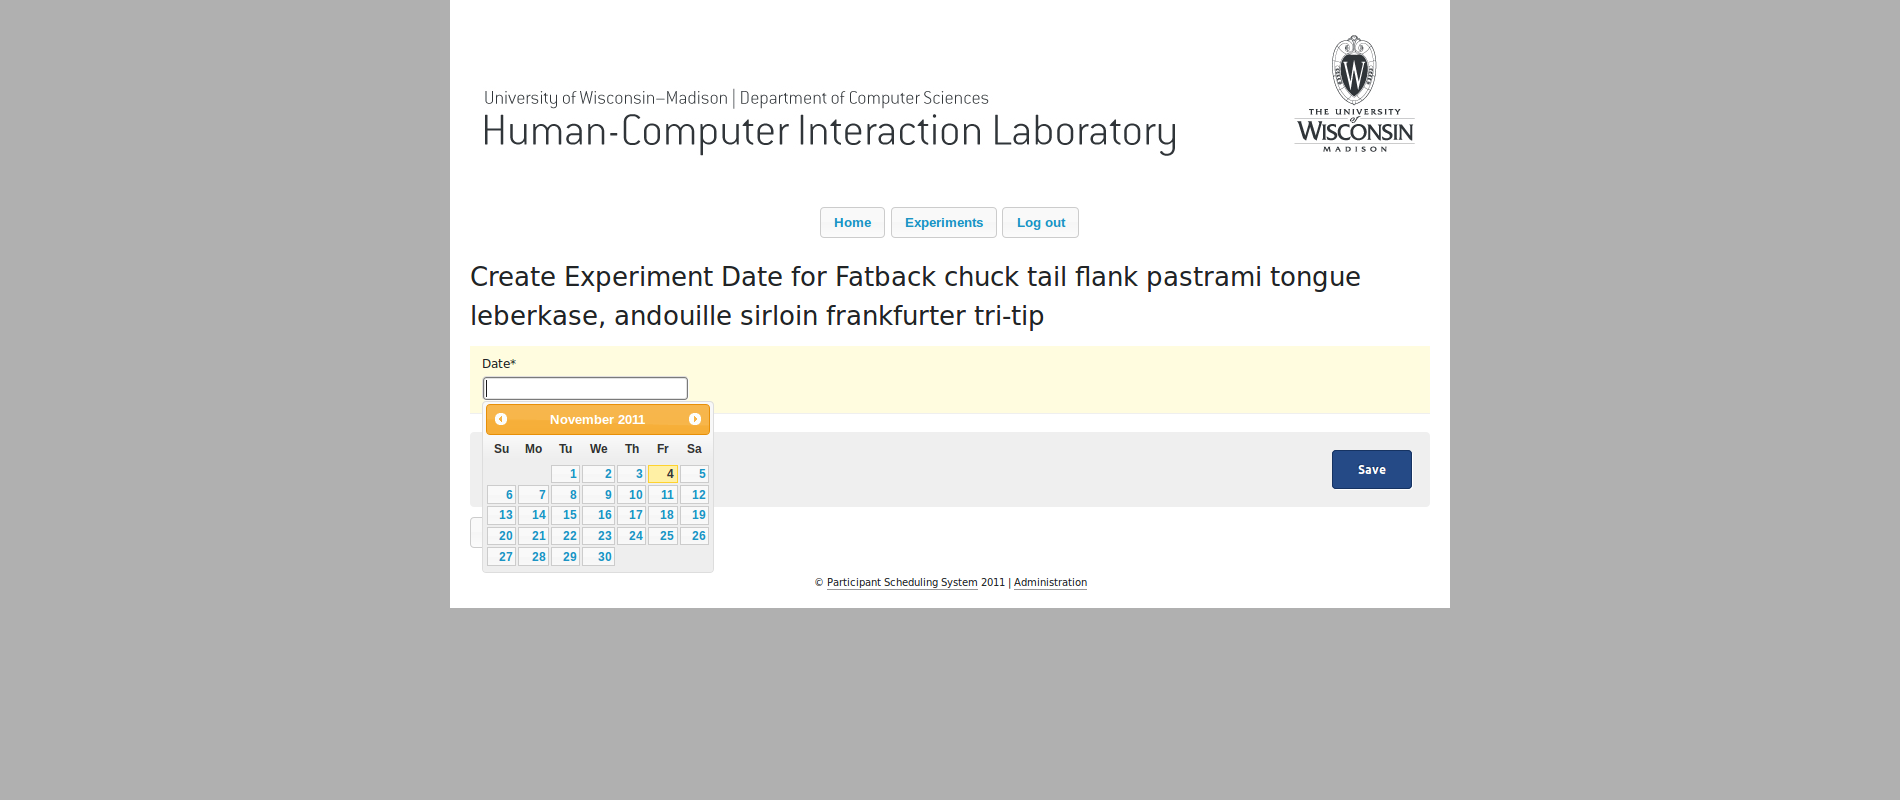
\includegraphics[width=6in]{../other/initial-interface-design/create-experiment-date.png}
\subsubsection{Revised}
The user will be able to type in a date manually without using the calendar widget. Help text explaining the date format will be added. The widget will not automatically appear on page load. It will be clear that the cancel button discards all unsaved changes.

\subsection{Edit Experiment Date}
\subsubsection{Initial}
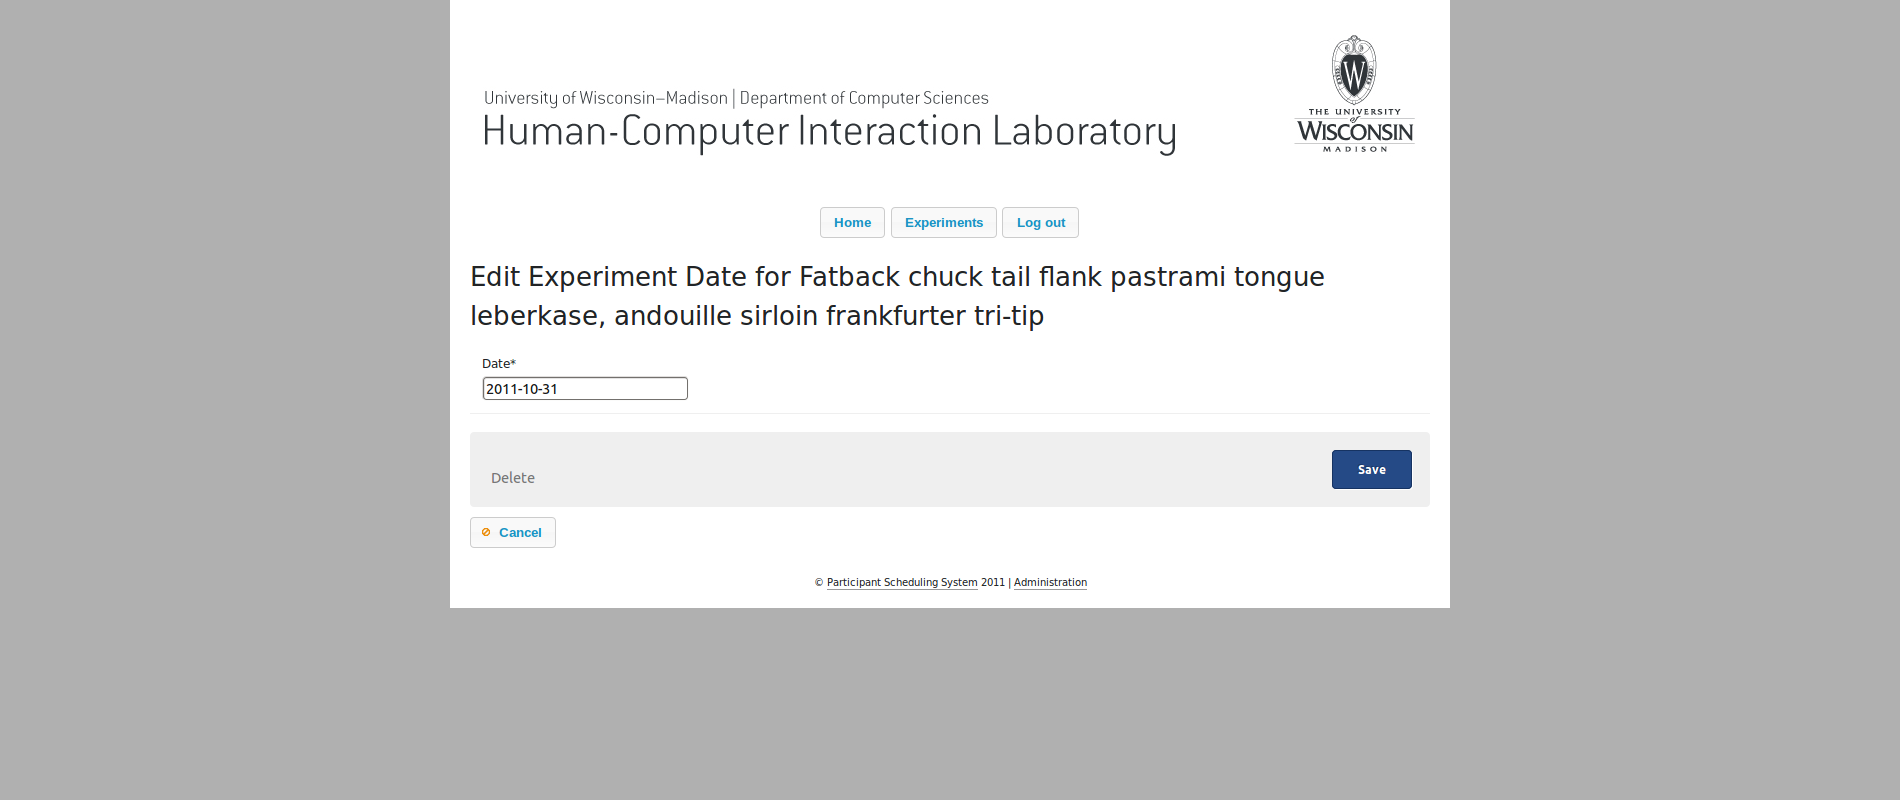
\includegraphics[width=6in]{../other/initial-interface-design/edit-experiment-date.png}
\subsubsection{Revised}
The delete button will not be so subtle. Also, see {\bf Create Experiment Date}.

\subsection{Delete Experiment Date}
\subsubsection{Initial}
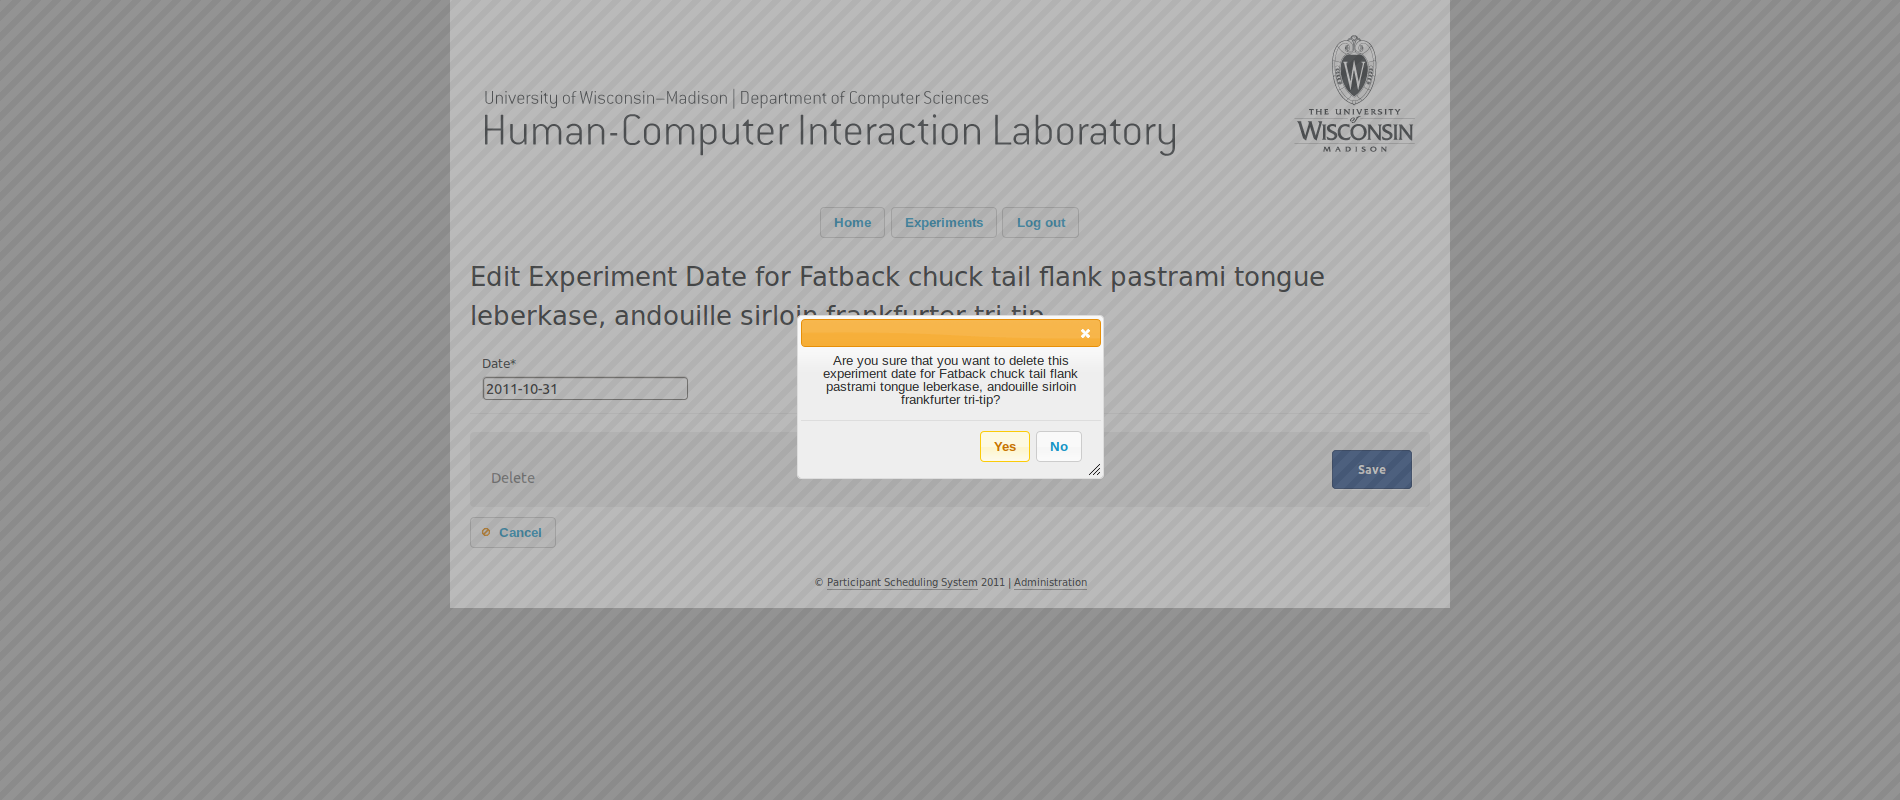
\includegraphics[width=6in]{../other/initial-interface-design/delete-experiment-date.png}
\subsubsection{Revised}
The jQueryUI CSS theme will match the existing CSS, so the dialog box will not appear so out of place.

\subsection{Experiment Date Time Ranges}
\subsubsection{Initial}
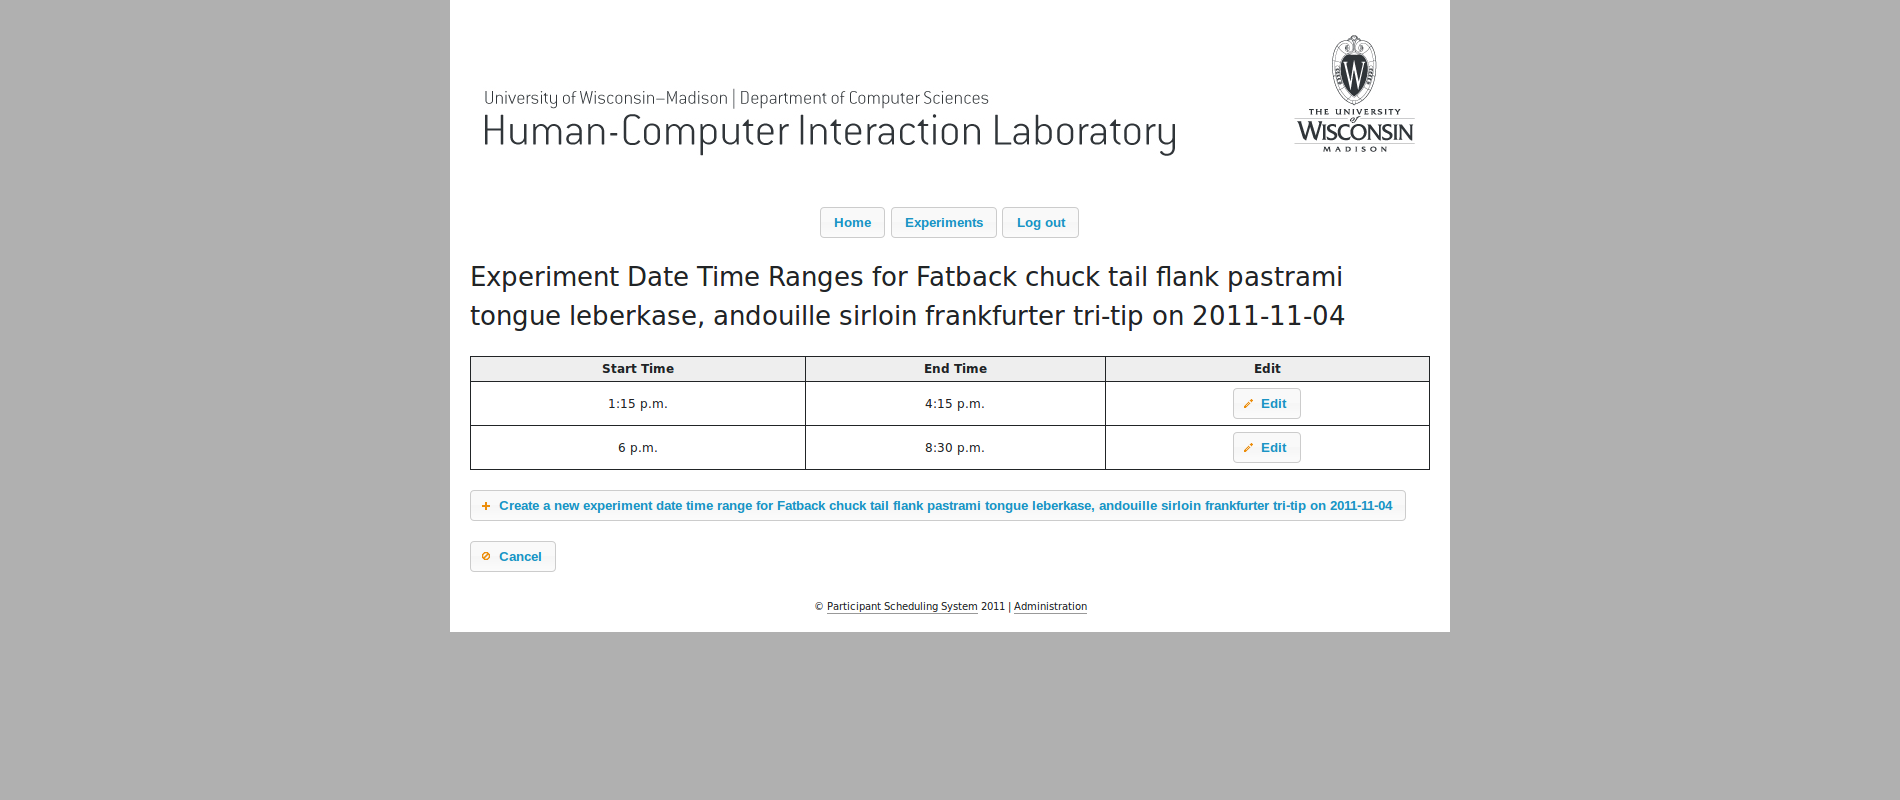
\includegraphics[width=6in]{../other/initial-interface-design/experiment-date-time-ranges.png}
\subsubsection{Revised}
The table will be filterable and sortable. Experiment date time ranges will be able to be mass-deleted from the table. The create button will be duplicated above the table as well. The cancel button will be changed to a back button with an appropriate icon.

\subsection{Create Experiment Date Time Range}
\subsubsection{Initial}
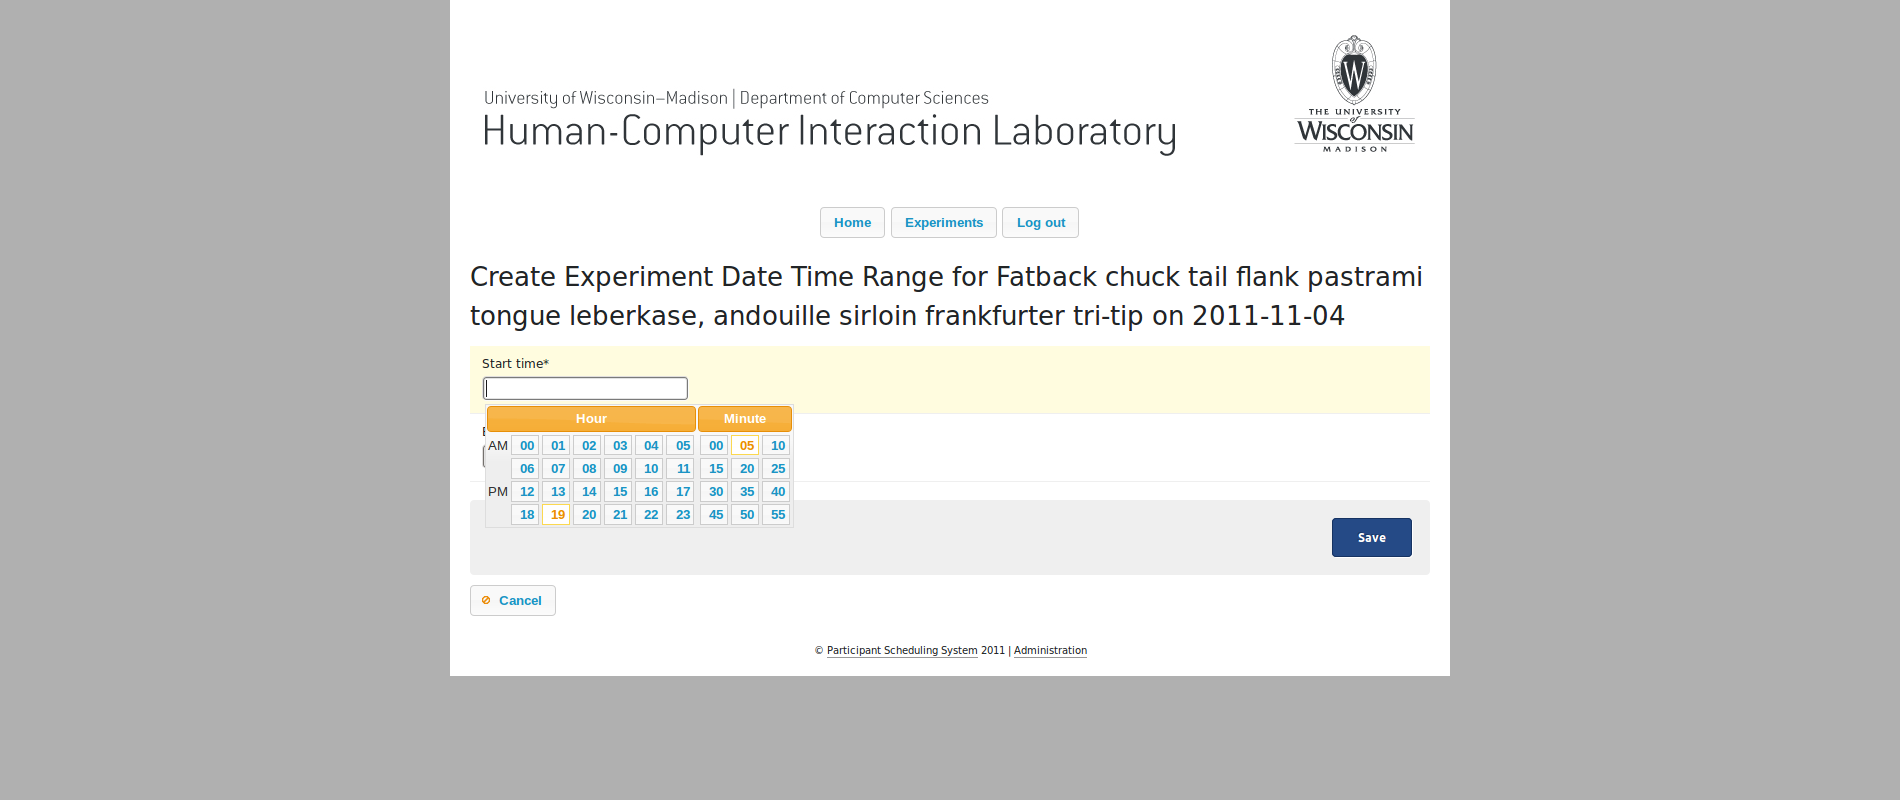
\includegraphics[width=6in]{../other/initial-interface-design/create-experiment-date-time-range.png}
\subsubsection{Revised}
The time widget will not have the AM or PM labels since it uses 24-hour time. Help text explaining the time format will be added. The widget will not automatically appear on page load. It will be clear that the cancel button discards all unsaved changes.

\subsection{Edit Experiment Date Time Range}
\subsubsection{Initial}
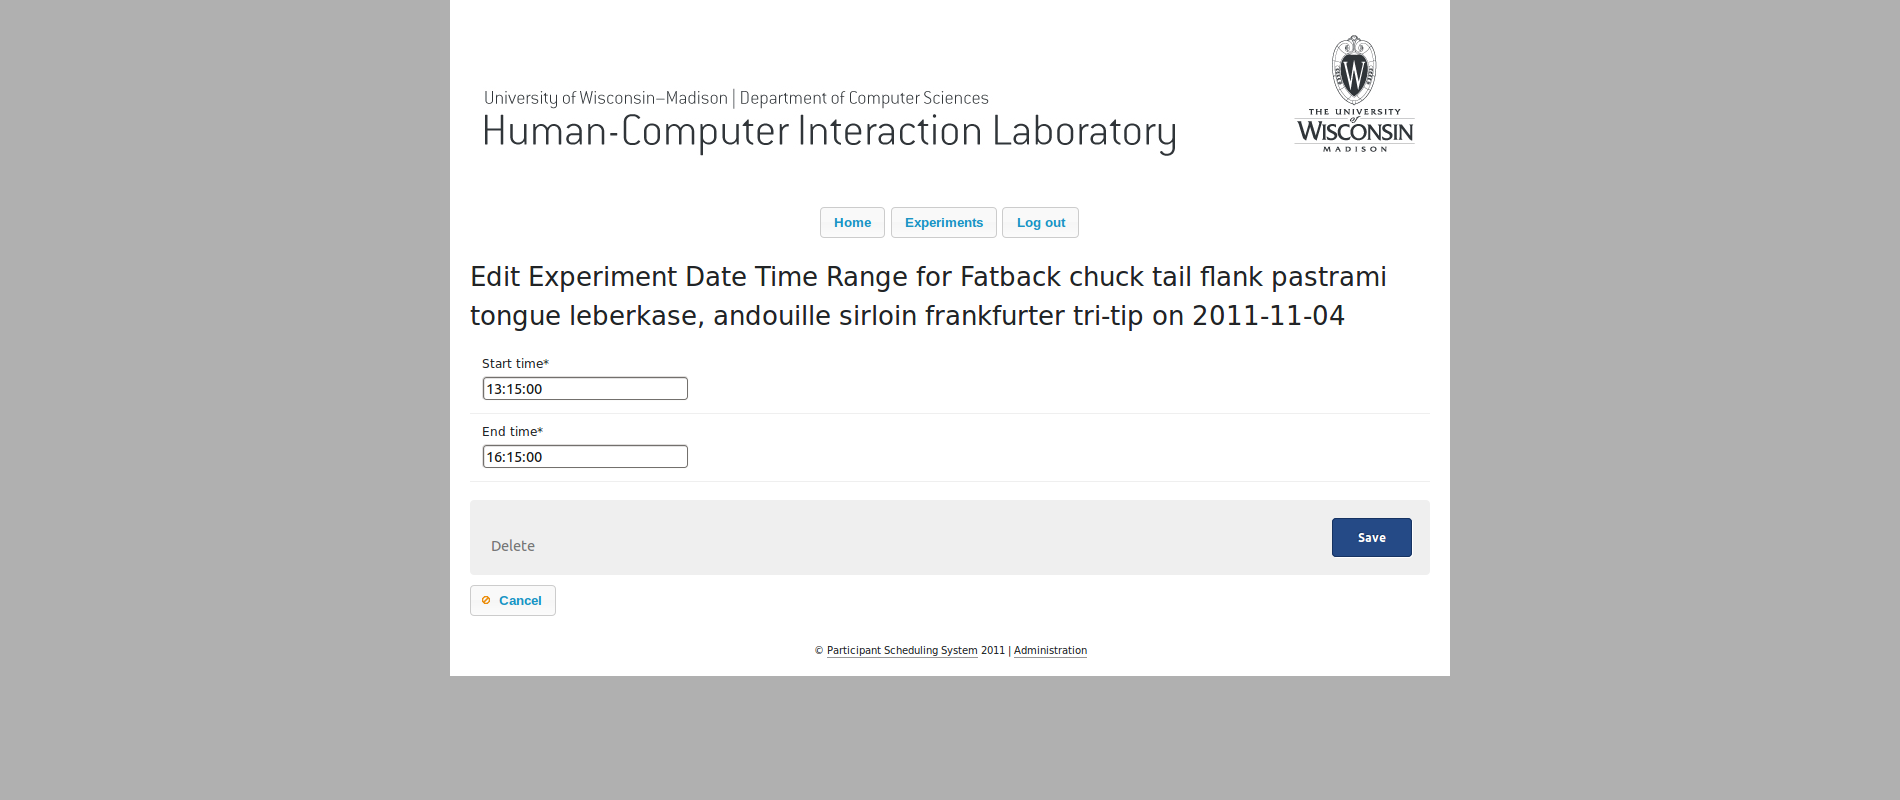
\includegraphics[width=6in]{../other/initial-interface-design/edit-experiment-date-time-range.png}
\subsubsection{Revised}
The delete button will not be so subtle. Also, see {\bf Create Experiment Date Time Range}.

\subsection{Delete Experiment Date Time Range}
\subsubsection{Initial}
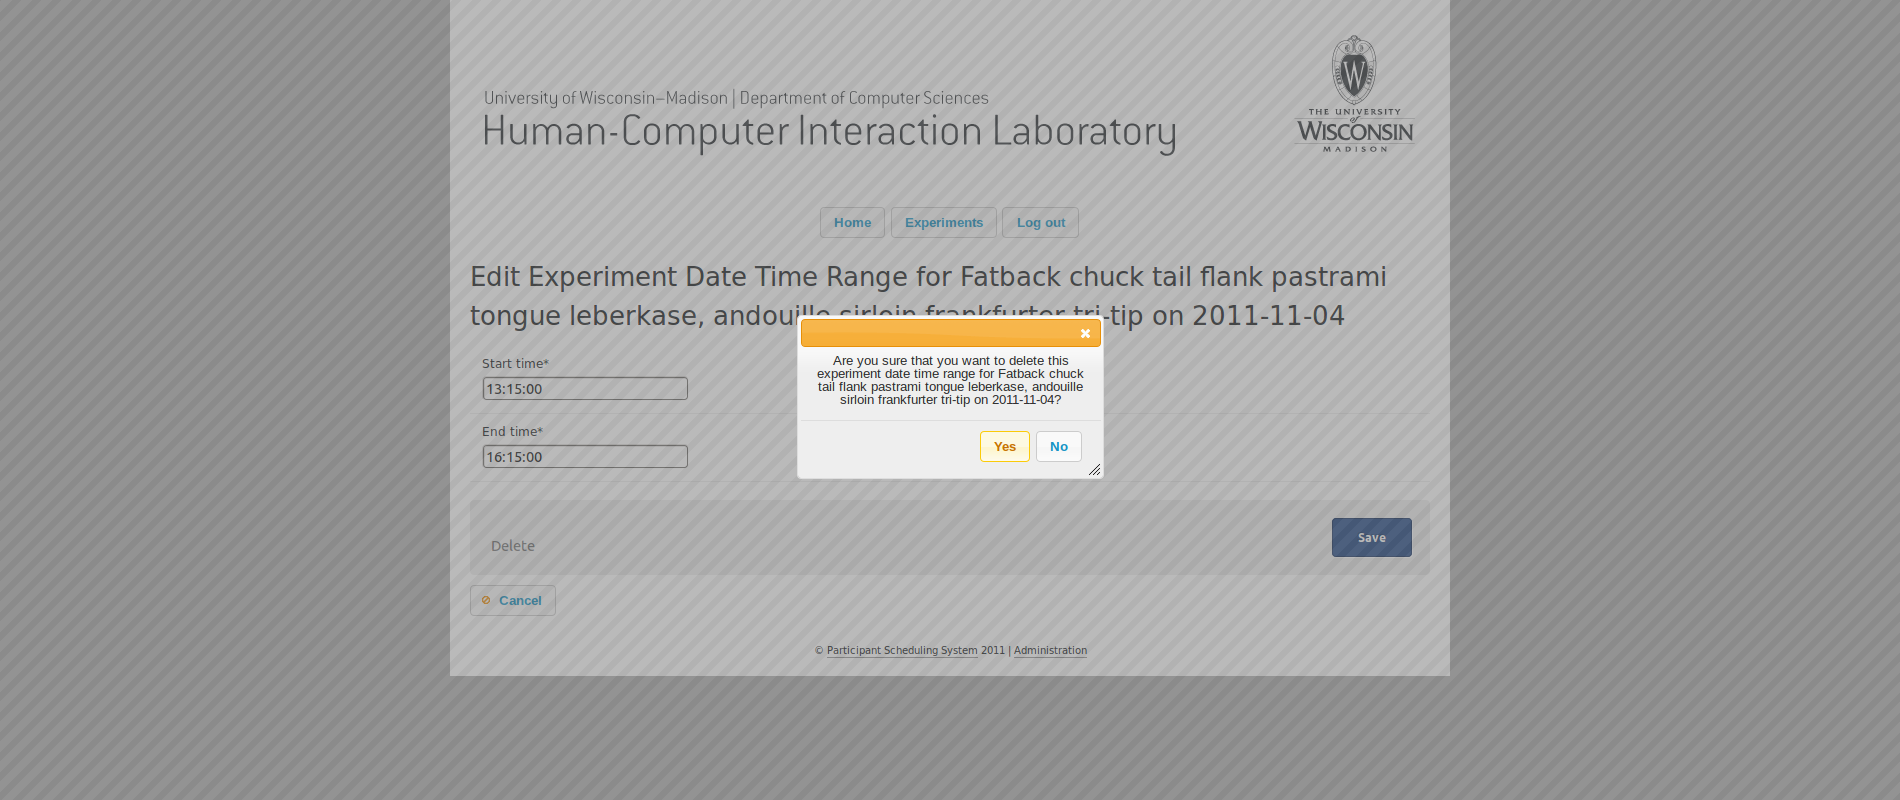
\includegraphics[width=6in]{../other/initial-interface-design/delete-experiment-date-time-range.png}
\subsubsection{Revised}
The jQueryUI CSS theme will match the existing CSS, so the dialog box will not appear so out of place.
